% Options for packages loaded elsewhere
\PassOptionsToPackage{unicode}{hyperref}
\PassOptionsToPackage{hyphens}{url}
%
\documentclass[
  ignorenonframetext,
]{beamer}
\usepackage{pgfpages}
\setbeamertemplate{caption}[numbered]
\setbeamertemplate{caption label separator}{: }
\setbeamercolor{caption name}{fg=normal text.fg}
\beamertemplatenavigationsymbolsempty
% Prevent slide breaks in the middle of a paragraph
\widowpenalties 1 10000
\raggedbottom
\setbeamertemplate{part page}{
  \centering
  \begin{beamercolorbox}[sep=16pt,center]{part title}
    \usebeamerfont{part title}\insertpart\par
  \end{beamercolorbox}
}
\setbeamertemplate{section page}{
  \centering
  \begin{beamercolorbox}[sep=12pt,center]{part title}
    \usebeamerfont{section title}\insertsection\par
  \end{beamercolorbox}
}
\setbeamertemplate{subsection page}{
  \centering
  \begin{beamercolorbox}[sep=8pt,center]{part title}
    \usebeamerfont{subsection title}\insertsubsection\par
  \end{beamercolorbox}
}
\AtBeginPart{
  \frame{\partpage}
}
\AtBeginSection{
  \ifbibliography
  \else
    \frame{\sectionpage}
  \fi
}
\AtBeginSubsection{
  \frame{\subsectionpage}
}
\usepackage{lmodern}
\usepackage{amssymb,amsmath}
\usepackage{ifxetex,ifluatex}
\ifnum 0\ifxetex 1\fi\ifluatex 1\fi=0 % if pdftex
  \usepackage[T1]{fontenc}
  \usepackage[utf8]{inputenc}
  \usepackage{textcomp} % provide euro and other symbols
\else % if luatex or xetex
  \usepackage{unicode-math}
  \defaultfontfeatures{Scale=MatchLowercase}
  \defaultfontfeatures[\rmfamily]{Ligatures=TeX,Scale=1}
\fi
\usetheme[]{Hannover}
\usecolortheme{dove}
\usefonttheme{structurebold}
% Use upquote if available, for straight quotes in verbatim environments
\IfFileExists{upquote.sty}{\usepackage{upquote}}{}
\IfFileExists{microtype.sty}{% use microtype if available
  \usepackage[]{microtype}
  \UseMicrotypeSet[protrusion]{basicmath} % disable protrusion for tt fonts
}{}
\makeatletter
\@ifundefined{KOMAClassName}{% if non-KOMA class
  \IfFileExists{parskip.sty}{%
    \usepackage{parskip}
  }{% else
    \setlength{\parindent}{0pt}
    \setlength{\parskip}{6pt plus 2pt minus 1pt}}
}{% if KOMA class
  \KOMAoptions{parskip=half}}
\makeatother
\usepackage{xcolor}
\IfFileExists{xurl.sty}{\usepackage{xurl}}{} % add URL line breaks if available
\IfFileExists{bookmark.sty}{\usepackage{bookmark}}{\usepackage{hyperref}}
\hypersetup{
  pdftitle={Session 6: Survival Analysis I},
  pdfauthor={Levi Waldron},
  hidelinks,
  pdfcreator={LaTeX via pandoc}}
\urlstyle{same} % disable monospaced font for URLs
\newif\ifbibliography
\usepackage{color}
\usepackage{fancyvrb}
\newcommand{\VerbBar}{|}
\newcommand{\VERB}{\Verb[commandchars=\\\{\}]}
\DefineVerbatimEnvironment{Highlighting}{Verbatim}{commandchars=\\\{\}}
% Add ',fontsize=\small' for more characters per line
\usepackage{framed}
\definecolor{shadecolor}{RGB}{248,248,248}
\newenvironment{Shaded}{\begin{snugshade}}{\end{snugshade}}
\newcommand{\AlertTok}[1]{\textcolor[rgb]{0.94,0.16,0.16}{#1}}
\newcommand{\AnnotationTok}[1]{\textcolor[rgb]{0.56,0.35,0.01}{\textbf{\textit{#1}}}}
\newcommand{\AttributeTok}[1]{\textcolor[rgb]{0.77,0.63,0.00}{#1}}
\newcommand{\BaseNTok}[1]{\textcolor[rgb]{0.00,0.00,0.81}{#1}}
\newcommand{\BuiltInTok}[1]{#1}
\newcommand{\CharTok}[1]{\textcolor[rgb]{0.31,0.60,0.02}{#1}}
\newcommand{\CommentTok}[1]{\textcolor[rgb]{0.56,0.35,0.01}{\textit{#1}}}
\newcommand{\CommentVarTok}[1]{\textcolor[rgb]{0.56,0.35,0.01}{\textbf{\textit{#1}}}}
\newcommand{\ConstantTok}[1]{\textcolor[rgb]{0.00,0.00,0.00}{#1}}
\newcommand{\ControlFlowTok}[1]{\textcolor[rgb]{0.13,0.29,0.53}{\textbf{#1}}}
\newcommand{\DataTypeTok}[1]{\textcolor[rgb]{0.13,0.29,0.53}{#1}}
\newcommand{\DecValTok}[1]{\textcolor[rgb]{0.00,0.00,0.81}{#1}}
\newcommand{\DocumentationTok}[1]{\textcolor[rgb]{0.56,0.35,0.01}{\textbf{\textit{#1}}}}
\newcommand{\ErrorTok}[1]{\textcolor[rgb]{0.64,0.00,0.00}{\textbf{#1}}}
\newcommand{\ExtensionTok}[1]{#1}
\newcommand{\FloatTok}[1]{\textcolor[rgb]{0.00,0.00,0.81}{#1}}
\newcommand{\FunctionTok}[1]{\textcolor[rgb]{0.00,0.00,0.00}{#1}}
\newcommand{\ImportTok}[1]{#1}
\newcommand{\InformationTok}[1]{\textcolor[rgb]{0.56,0.35,0.01}{\textbf{\textit{#1}}}}
\newcommand{\KeywordTok}[1]{\textcolor[rgb]{0.13,0.29,0.53}{\textbf{#1}}}
\newcommand{\NormalTok}[1]{#1}
\newcommand{\OperatorTok}[1]{\textcolor[rgb]{0.81,0.36,0.00}{\textbf{#1}}}
\newcommand{\OtherTok}[1]{\textcolor[rgb]{0.56,0.35,0.01}{#1}}
\newcommand{\PreprocessorTok}[1]{\textcolor[rgb]{0.56,0.35,0.01}{\textit{#1}}}
\newcommand{\RegionMarkerTok}[1]{#1}
\newcommand{\SpecialCharTok}[1]{\textcolor[rgb]{0.00,0.00,0.00}{#1}}
\newcommand{\SpecialStringTok}[1]{\textcolor[rgb]{0.31,0.60,0.02}{#1}}
\newcommand{\StringTok}[1]{\textcolor[rgb]{0.31,0.60,0.02}{#1}}
\newcommand{\VariableTok}[1]{\textcolor[rgb]{0.00,0.00,0.00}{#1}}
\newcommand{\VerbatimStringTok}[1]{\textcolor[rgb]{0.31,0.60,0.02}{#1}}
\newcommand{\WarningTok}[1]{\textcolor[rgb]{0.56,0.35,0.01}{\textbf{\textit{#1}}}}
\usepackage{graphicx,grffile}
\makeatletter
\def\maxwidth{\ifdim\Gin@nat@width>\linewidth\linewidth\else\Gin@nat@width\fi}
\def\maxheight{\ifdim\Gin@nat@height>\textheight\textheight\else\Gin@nat@height\fi}
\makeatother
% Scale images if necessary, so that they will not overflow the page
% margins by default, and it is still possible to overwrite the defaults
% using explicit options in \includegraphics[width, height, ...]{}
\setkeys{Gin}{width=\maxwidth,height=\maxheight,keepaspectratio}
% Set default figure placement to htbp
\makeatletter
\def\fps@figure{htbp}
\makeatother
\setlength{\emergencystretch}{3em} % prevent overfull lines
\providecommand{\tightlist}{%
  \setlength{\itemsep}{0pt}\setlength{\parskip}{0pt}}
\setcounter{secnumdepth}{-\maxdimen} % remove section numbering

\title{Session 6: Survival Analysis I}
\author{Levi Waldron}
\date{}
\institute{CUNY SPH Biostatistics 2}

\begin{document}
\frame{\titlepage}

\hypertarget{learning-objectives-and-outline}{%
\section{Learning objectives and
outline}\label{learning-objectives-and-outline}}

\begin{frame}{Learning objectives}
\protect\hypertarget{learning-objectives}{}

\begin{enumerate}
\tightlist
\item
  Distinguish censored data from binary or continuous data
\item
  Define survival function, hazard functions, cumulative event function
\item
  Perform a Kaplan-Meier estimate
\item
  Perform, interpret, and identify assumptions of the logrank test
\item
  Define \textbf{potential follow-up time}
\item
  Calculate median survival time and potential follow-up time
\end{enumerate}

\end{frame}

\begin{frame}{Outline}
\protect\hypertarget{outline}{}

\begin{enumerate}
\tightlist
\item
  Introduction to censored data

  \begin{itemize}
  \tightlist
  \item
    Outcome variable: time-to-event
  \item
    Censored data
  \end{itemize}
\item
  Survival function and Kaplan-Meier estimator
\item
  Comparing groups: Log-rank test
\end{enumerate}

\begin{itemize}
\tightlist
\item
  Vittinghoff sections 3.1-3.5
\end{itemize}

\end{frame}

\hypertarget{introduction-to-censored-data}{%
\section{Introduction to censored
data}\label{introduction-to-censored-data}}

\begin{frame}{Outcome variable: time to event}
\protect\hypertarget{outcome-variable-time-to-event}{}

\begin{itemize}
\tightlist
\item
  Generally time to the occurrence of a particular event, e.g.~

  \begin{itemize}
  \tightlist
  \item
    death
  \item
    disease recurrence
  \item
    or other experience of interest
  \end{itemize}
\item
  Time: The time from the beginning of an observation period t0
  (e.g.~surgery) to:

  \begin{itemize}
  \tightlist
  \item
    an event, or
  \item
    end of the study, or
  \item
    loss of contact or withdrawal from the study
  \end{itemize}
\end{itemize}

\end{frame}

\begin{frame}{Typical research questions}
\protect\hypertarget{typical-research-questions}{}

\begin{itemize}
\tightlist
\item
  What is the median survival time (in years) of patients diagnosed with
  a certain disease?
\item
  What is the probability of those patients surviving for at least 5
  years?
\item
  Are certain personal, behavioral, or clinical characteristics
  correlated with participant's chance of survival?
\item
  Is there a survival difference between groups?

  \begin{itemize}
  \tightlist
  \item
    e.g.~treatment vs.~control
  \item
    e.g.~exposed vs.~unexposed
  \end{itemize}
\end{itemize}

\end{frame}

\begin{frame}{Special considerations in survival analysis}
\protect\hypertarget{special-considerations-in-survival-analysis}{}

\begin{itemize}
\tightlist
\item
  Survival data requires special techniques:

  \begin{itemize}
  \tightlist
  \item
    Survival data is generally not normally distributed
  \item
    \textbf{Censoring} - observe individuals for differing lengths of
    time that may or may not result in an ``event''
  \end{itemize}
\item
  Censoring is a key challenge in survival analysis. Consider a clinical
  study where:

  \begin{itemize}
  \tightlist
  \item
    patient 1 dies 1 month after diagnosis
  \item
    patient 2 dies 12 years after diagnosis
  \item
    patient 3 is lost to follow-up after 1 month
  \item
    patient 4 is still alive after 12 years of follow-up
  \end{itemize}
\end{itemize}

\emph{Question \#1: which patients are ``censored?''}

\emph{Question \#2: how would you rank these patients in order of
disease severity?}

\end{frame}

\begin{frame}{Definitions}
\protect\hypertarget{definitions}{}

\emph{Definition}: A survival time is said to be \emph{right-censored}
at time t if it is only known to be greater than t.

\emph{Definition}: The \emph{survival function} at time t, denoted
\(S(t)\), is the probability of being event-free at t. Equivalently, it
is the probability that the survival time is greater than t.

\end{frame}

\begin{frame}[fragile]{leukemia Example: see leuk.csv}
\protect\hypertarget{leukemia-example-see-leuk.csv}{}

\begin{itemize}
\tightlist
\item
  Study of 6-mercaptopurine (6-MP) maintenance therapy for children in
  remission from acute lymphoblastic leukemia (ALL)
\item
  42 patients achieved remission from induction therapy and were then
  randomized in equal numbers to 6-MP or placebo.
\item
  Survival time studied was from randomization until relapse.
\end{itemize}

Survival times in weeks for Placebo group:

\begin{verbatim}
##  [1]  1  1  2  2  3  4  4  5  5  8  8  8  8 11 11 12 12 15 17 22 23
\end{verbatim}

Survival times in weeks for Treatment group:

\begin{verbatim}
##  [1]  6   6   6   7  10  13  16  22  23   6+  9+ 10+ 11+ 17+ 19+ 20+ 25+ 32+ 32+
## [20] 34+ 35+
\end{verbatim}

\end{frame}

\begin{frame}{A graphical look at the treatment group}
\protect\hypertarget{a-graphical-look-at-the-treatment-group}{}

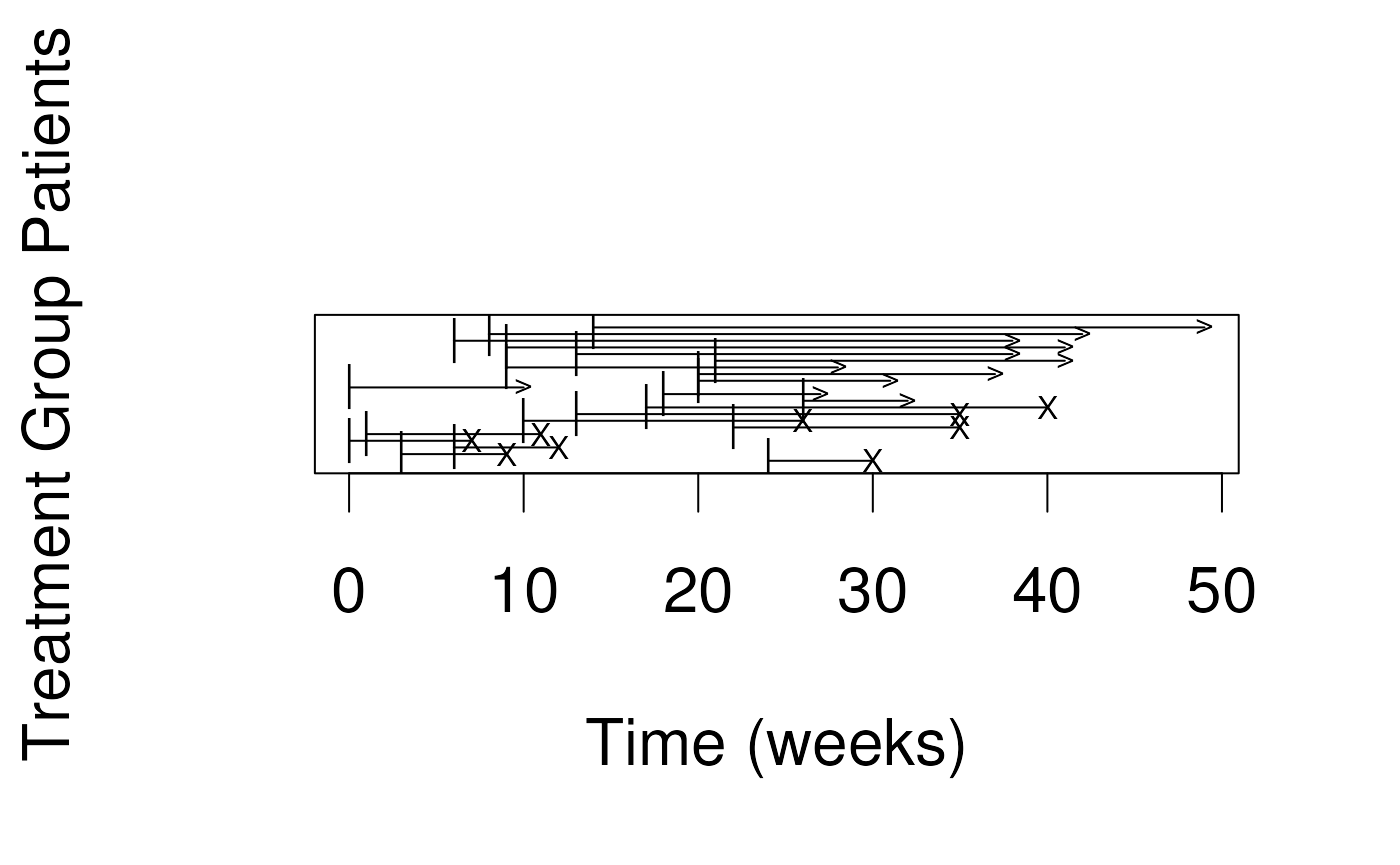
\includegraphics{../docs/articles/session_lecture_files/figure-beamer/unnamed-chunk-3-1.pdf}

(Initiation times (t0) are simulated between 0 and 26 weeks)

\end{frame}

\begin{frame}{leukemia study follow-up table}
\protect\hypertarget{leukemia-study-follow-up-table}{}

\begin{figure}
\centering
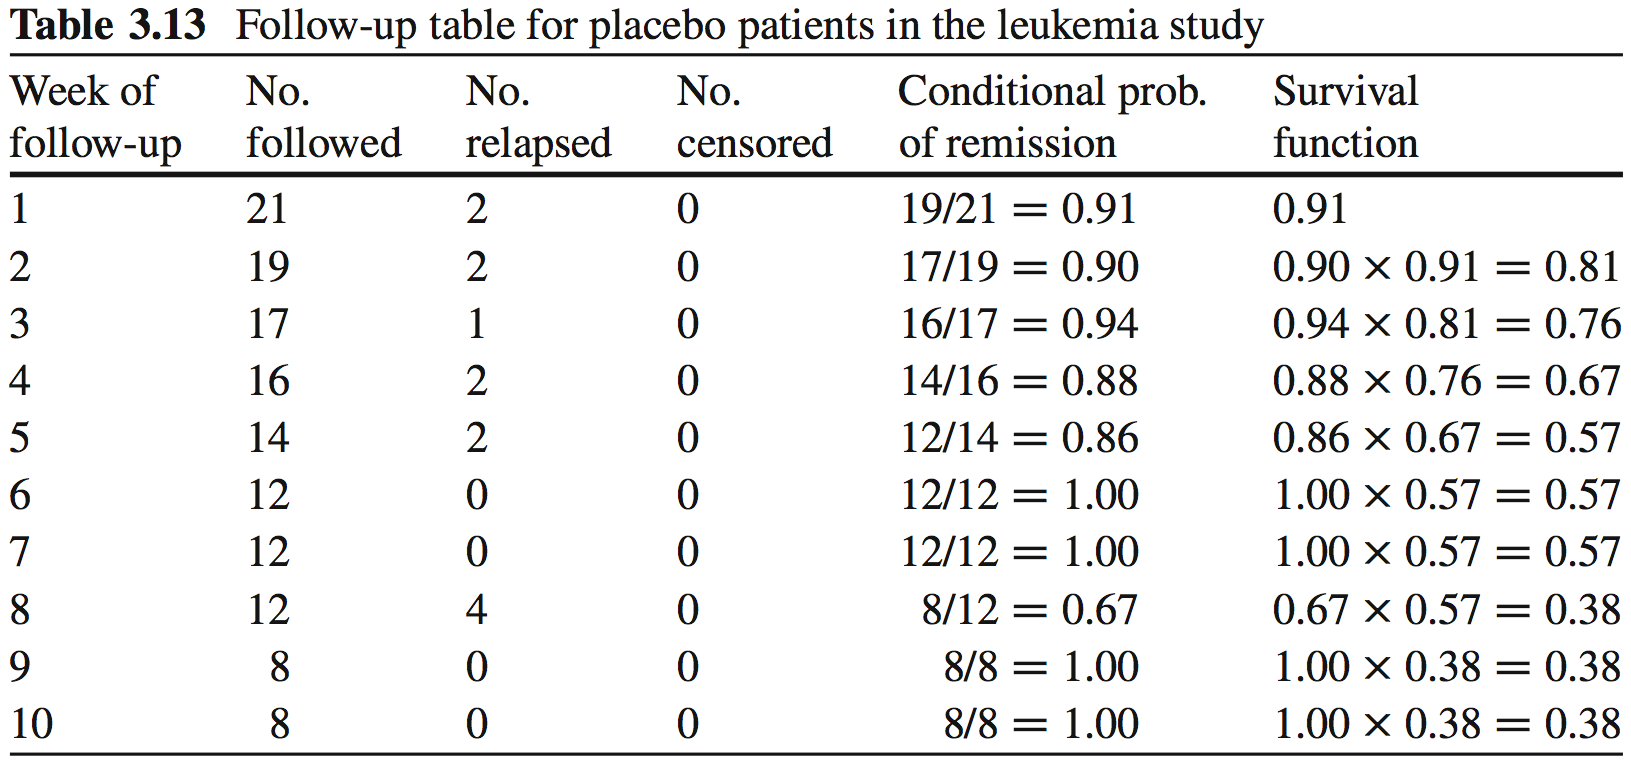
\includegraphics{figures/leukemiatable.png}
\caption{leukemia Follow-up Table}
\end{figure}

This is the \textbf{Kaplan-Meier Estimate} \(\hat S(t)\) of the Survival
function \(S(t)\).

\end{frame}

\hypertarget{survival-function-and-kaplan-meier-estimator}{%
\section{Survival function and Kaplan-Meier
estimator}\label{survival-function-and-kaplan-meier-estimator}}

\begin{frame}[fragile]{Kaplan-Meier Estimate vs.~time}
\protect\hypertarget{kaplan-meier-estimate-vs.-time}{}

\begin{verbatim}
## Warning: Vectorized input to `element_text()` is not officially supported.
## Results may be unexpected or may change in future versions of ggplot2.
\end{verbatim}

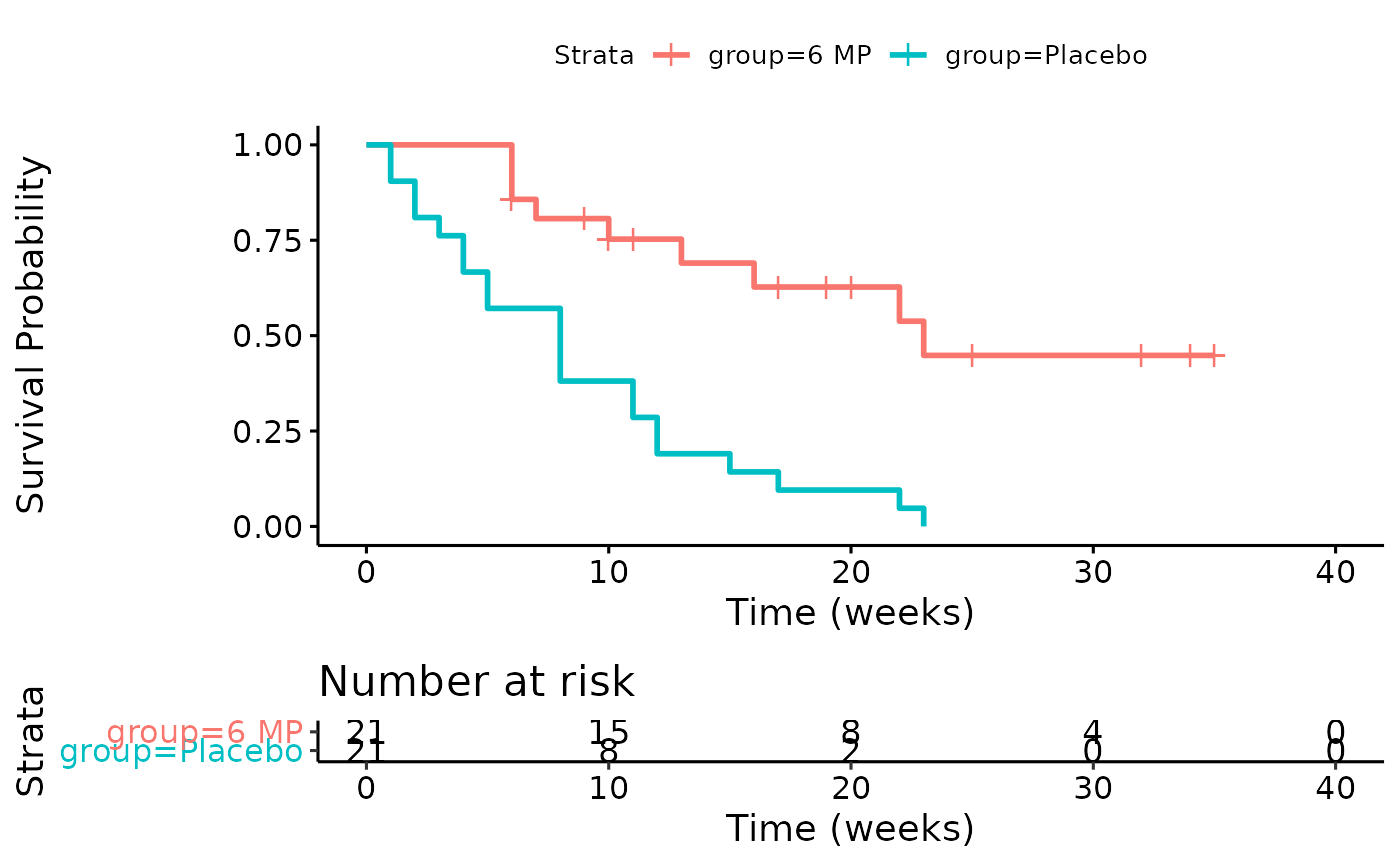
\includegraphics{../docs/articles/session_lecture_files/figure-beamer/unnamed-chunk-4-1.pdf}

\end{frame}

\begin{frame}[fragile]{Median Survival Time}
\protect\hypertarget{median-survival-time}{}

\emph{Definition}: \emph{Median Survival Time} is the time at which half
of a group (sample, population) is expected to experience an event (in
this example, death)

\begin{itemize}
\tightlist
\item
  Without censoring, median survival time can be calculated the obvious
  way
\item
  With censoring, we need to use the Kaplan-Meier estimate of the
  survival function \(\hat S(t)\)
\end{itemize}

\footnotesize

\begin{Shaded}
\begin{Highlighting}[]
\KeywordTok{survfit}\NormalTok{(}\KeywordTok{Surv}\NormalTok{(time, cens)}\OperatorTok{~}\NormalTok{group, }\DataTypeTok{data=}\NormalTok{leuk)}
\end{Highlighting}
\end{Shaded}

\begin{verbatim}
## Call: survfit(formula = Surv(time, cens) ~ group, data = leuk)
## 
##                n events median 0.95LCL 0.95UCL
## group=6 MP    21      9     23      16      NA
## group=Placebo 21     21      8       4      12
\end{verbatim}

\end{frame}

\begin{frame}[fragile]{Median Potential Follow-Up Time}
\protect\hypertarget{median-potential-follow-up-time}{}

\emph{Definition}: \emph{Median Potential Follow-Up Time} is the time
for which half of a sample would have been expected to be followe,
\emph{in the absence of events}.

\begin{itemize}
\tightlist
\item
  Without any events, median follow-up time can be calculated the
  obvious way
\item
  With events, a simple median will \emph{under-estimate} the potential
  follow-up time. Use a reverse Kaplan-Meier estimate instead:
\end{itemize}

\footnotesize

\begin{Shaded}
\begin{Highlighting}[]
\KeywordTok{survfit}\NormalTok{(}\KeywordTok{Surv}\NormalTok{(time, }\DecValTok{1}\OperatorTok{-}\NormalTok{cens)}\OperatorTok{~}\NormalTok{group, }\DataTypeTok{data=}\NormalTok{leuk)}
\end{Highlighting}
\end{Shaded}

\begin{verbatim}
## Call: survfit(formula = Surv(time, 1 - cens) ~ group, data = leuk)
## 
##                n events median 0.95LCL 0.95UCL
## group=6 MP    21     12     25      17      NA
## group=Placebo 21      0     NA      NA      NA
\end{verbatim}

\emph{Note}: \emph{Actual} median follow-up time is half as long for the
placebo group, but there is not reason to believe the potential
follow-up times were different

\end{frame}

\begin{frame}{Cumulative Event Function}
\protect\hypertarget{cumulative-event-function}{}

\emph{Definition}: The \emph{cumulative event function} at time t,
denoted \(F(t)\), is the probability that the event has occurred by time
t, or equivalently, the probability that the survival time is less than
or equal to t. Note \(F(t) = 1-S(t)\).

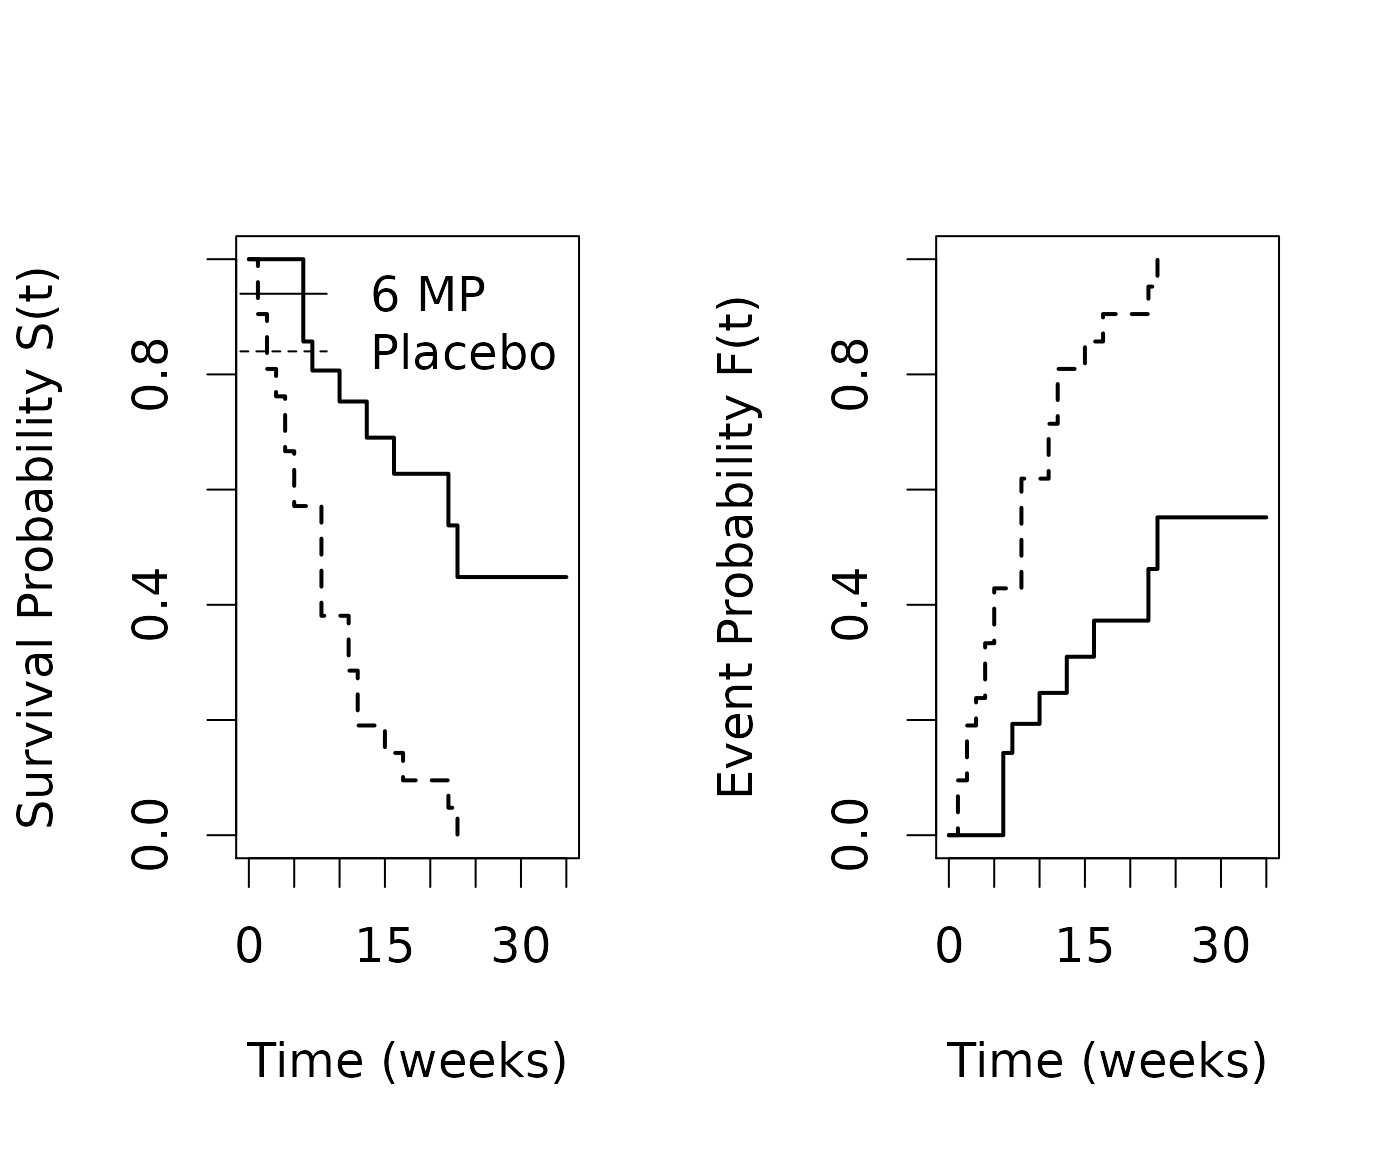
\includegraphics{../docs/articles/session_lecture_files/figure-beamer/unnamed-chunk-7-1.pdf}

\end{frame}

\begin{frame}{Hazard and Cumulative Hazard functions}
\protect\hypertarget{hazard-and-cumulative-hazard-functions}{}

\begin{itemize}
\tightlist
\item
  \(h(t)\): hazard function, risk of event at a point in time

  \begin{itemize}
  \tightlist
  \item
    only calculated by software
  \end{itemize}
\item
  \(H(t) = -log[S(t)]\): cumulative hazard function

  \begin{itemize}
  \tightlist
  \item
    not easily interpretable
  \item
    cumulative force of mortality, or the number of events that would be
    expected for each individual by time t if the event were a
    repeatable process.
  \end{itemize}
\item
  Will be important next class for Cox Proportional Hazards
\end{itemize}

\end{frame}

\hypertarget{comparing-groups-using-the-logrank-test}{%
\section{Comparing Groups Using the Logrank
Test}\label{comparing-groups-using-the-logrank-test}}

\begin{frame}{Comparing Groups Using the Logrank Test}

\begin{itemize}
\tightlist
\item
  \emph{logrank test} is used to compare survival between two or more
  groups

  \begin{itemize}
  \tightlist
  \item
    \(H_0\) is that the population survival functions are equal at all
    follow-up times
  \item
    \(H_1\) is that the population survival functions differ at at least
    one follow-up time
  \end{itemize}
\item
  logrank test is really just a \emph{chi-square test} comparing
  expected vs.~observed number of events in each group.

  \begin{itemize}
  \tightlist
  \item
    Observed is just what we see.
  \item
    How to calculate expected?
  \end{itemize}
\end{itemize}

\end{frame}

\hypertarget{comparing-groups-log-rank-test}{%
\section{Comparing groups: Log-rank
test}\label{comparing-groups-log-rank-test}}

\begin{frame}[fragile]{Setting for the Logrank Test}
\protect\hypertarget{setting-for-the-logrank-test}{}

\(H_0\): The risk in two or more groups is the same. Observed
differences in numbers of events only occur by chance.

\footnotesize

\begin{Shaded}
\begin{Highlighting}[]
\KeywordTok{survdiff}\NormalTok{(}\KeywordTok{Surv}\NormalTok{(time, cens)}\OperatorTok{~}\NormalTok{group, }\DataTypeTok{data=}\NormalTok{leuk)}
\end{Highlighting}
\end{Shaded}

\begin{verbatim}
## Call:
## survdiff(formula = Surv(time, cens) ~ group, data = leuk)
## 
##                N Observed Expected (O-E)^2/E (O-E)^2/V
## group=6 MP    21        9     19.3      5.46      16.8
## group=Placebo 21       21     10.7      9.77      16.8
## 
##  Chisq= 16.8  on 1 degrees of freedom, p= 4e-05
\end{verbatim}

\begin{itemize}
\tightlist
\item
  Many alternatives are available, but log-rank should be the default
  unless you have good reason.

  \begin{itemize}
  \tightlist
  \item
    E.g. Wilcoxon (Breslow), Tarone-Ware, Peto tests
  \end{itemize}
\end{itemize}

\end{frame}

\begin{frame}{Notes about the Logrank Test}
\protect\hypertarget{notes-about-the-logrank-test}{}

\begin{itemize}
\tightlist
\item
  Non-parametric: no assumptions on the form of \(S(t)\)
\item
  Log-rank test and K-M curves don't work with continuous predictors
\item
  Assumes \emph{non-informative censoring}:

  \begin{itemize}
  \tightlist
  \item
    censoring is unrelated to the likelihood of developing the event of
    interest
  \item
    for each subject, his/her censoring time is statistically
    independent from their failure time
  \end{itemize}
\end{itemize}

\end{frame}

\hypertarget{summary}{%
\section{Summary}\label{summary}}

\begin{frame}{Summary}

\begin{itemize}
\tightlist
\item
  Censoring requires special methods to make full use of the data
\item
  Kaplan-Meier estimate provides non-parametric estimate of the survival
  function

  \begin{itemize}
  \tightlist
  \item
    non-parametric meaning that no form of the survival function is
    assumed; instead it is empirically estimated
  \end{itemize}
\item
  Logrank test provides a non-parametric hypothesis test

  \begin{itemize}
  \tightlist
  \item
    H0: identical survival functions of multiple strata
  \end{itemize}
\end{itemize}

\end{frame}

\end{document}
